\section{Анализ оптимизационного метода для квазистационарной модели}\label{sec:ch2/sec3}

\subsection{Formulation of an Optimal Control Problem}\label{subsec:ch2/sec3/subsec1}
квазистационарный радиационный и диффузионный теплообмен в ограниченной области
$\Omega \subset \mathrm{R}^{3}$ с границей $\Gamma=\partial \Omega$ моделируется
$P_{1}$-аппроксимацией для уравнения переноса излучения
со следующей начально-краевой задачей [16, 23]:

\[
\begin{gathered}
\frac{\partial \theta}{\partial t}-a \Delta \theta+b
\kappa_{a}\left(|\theta| \theta^{3}-\varphi\right)=0, \\
-\alpha \Delta \varphi+\kappa_{a}\left(\varphi-|\theta| \theta^{3}\right)=0,
\quad x \in \Omega, \quad 0<t<T; \\
a\left(\partial_{n} \theta+\theta\right)=r,
\quad \alpha\left(\partial_{n} \varphi+\varphi\right)=u \text { на } \Gamma; \\
\left.\theta\right|_{t=0}=\theta_{0}.
\end{gathered}
\]

Здесь $\theta$ — нормированная температура, $\varphi$ — нормированная интенсивность излучения,
усредненная по всем направлениям.
Положительные параметры $a, b, \kappa_{a}$ и $\alpha$, описывающие свойства среды,
определяются стандартным образом [18].
Задана функция $r(x, t), x \in \Gamma, t \in(0, T)$,
а неизвестная функция $u(x, t), x \in \Gamma, t \in$ $(0, T)$ — управление.
Через $\partial_{n}$ мы обозначаем производную по направлению внешней нормали $\mathbf{n}$.


Экстремальная задача состоит в том, чтобы найти тройку
$\left\{\theta_{\lambda}, \varphi_{\lambda}, u_{\lambda}\right\}$ такую, что

\[
J_{\lambda}(\theta, u)=\frac{1}{2} \int_{0}^{T}
\int_{\Gamma}\left(\theta-\theta_{b}\right)^{2} d \Gamma d t+\frac{\lambda}{2}
\int_{0}^{T} \int_{\Gamma} u^{2} d \Gamma d t \rightarrow \inf
\]
на решениях задачи (1)-(3).

Функция $\theta_{b}(x, t), x \in \Gamma, t \in(0, T)$,
а также регуляризирующий параметр $\lambda>0$ являются заданными.

Задача оптимального управления (1)-(4), если $r \coloneqq a\left(\theta_{b}+q_{b}\right)$,
где $q_{b}$ — заданная функция на $\Sigma =\Gamma \times(0, T)$,
является при малых значениях $\lambda$ аппроксимацией краевой задачи для уравнения (1),
для которого неизвестны граничные условия для интенсивности излучения $\varphi$.
Вместо них задаются граничные температура и внешний поток,
\[
\left.\theta\right|_{\Gamma}=\theta_{b},\left.\quad \partial_{n} \theta\right|_{\Gamma}=q_{b}.
\]

Математическое моделирование теплообмена с учетом радиационных эффектов используется в различных
приложениях, например, в электронно-микроскопической диагностике [22, 24],
производстве стекла [13, 14] и лазерной термотерапии [20].
Подробный теоретический и численный анализ различных постановок краевых и обратных задач,
а также задач управления для уравнений радиационного теплообмена в рамках $P_1$-приближения
для уравнения переноса излучения представлен в в [7, 11,16,18, 19,23].
Интересные краевые задачи, связанные с радиационным теплообменом,
изучаются в [2-6].
В [12] доказана нелокальная разрешимость нестационарных и стационарных
краевых задач для уравнений комплексного теплообмена без граничных
условий на интенсивность излучения и с условиями (5) на температуру.

Основные результаты работы заключаются в получении априорных оценок решения задачи (1), (2),
на основании которых доказывается разрешимость задачи оптимального управления (1)-(4)
и оптимальность система является производной.
Показано, что последовательность $\left\{\theta_{\lambda}, \varphi_{\lambda}, u_{\lambda}\right\}$
решений экстремальной задачи (1)-(4) при $ \lambda \rightarrow+0$
сходится к решению начально-краевой задачи (1), (5) с условиями типа Коши для температуры.
Представлен алгоритм решения задачи управления.

\subsection{Формализация задачи управления}\label{subsec:ch2/sec3/subsec2}
В дальнейшем предполагается, что $\Omega \subset \mathrm{R}^{3}$ — ограниченная строго липшицева область,
граница которой $\Gamma$ состоит из конечного числа гладких кусков.
Через $L^{s}, 1 \leq s \leq$ $\infty$
обозначается пространство Лебега, а через $H^{s}$ пространство Соболева $W_{2}^{s}$.
Пусть $H=$ $L^{2}(\Omega), V=H^{1}(\Omega)$.
Через $V^{\prime}$ обозначим двойственное к $V$ пространство, а через $L^{s}(0, T; X)$
пространство Лебега функций из $L^{s}$, определенных на $(0, T)$ со значениями в пространстве $X$.
Пространство $H$ отождествляется с пространством
$H^{\prime}$ так, что $V \subset H=H^{\prime} \subset V^{\prime}$.
Обозначим через $\|\cdot\|$ стандартную норму в $H$, а через $(f, v)$
значение функционала $f \in V^{\prime}$ в элементе $v \in V$,
что совпадает со скалярным произведением в $H$, если $f \in H$.

Через $U$ обозначим пространство $L^{2}(\Sigma)$ с нормой

\[ \|u\|_{\Sigma}=\left(\int_{\Sigma} u^{2} d \Gamma d t\right)^{1 / 2}. \]

Мы также будем использовать пространство
$W=\left\{y \in L^{2}(0, T ; V): \quad y^{\prime}
\in L^{2}\left(0, T, V^{\prime}\right)\right\}$,
где $y^{\prime}=d y / d t$.

Будем считать, что
(i) $a, b, \alpha, \kappa_{a}, \lambda=$ Const $>0$,
(ii) $\theta_{b}, q_{b} \in U, r=a\left(\theta_{b}+q_{b}\right) \in L^{5}(\Sigma) \theta_{0} \in L^{5}(\Omega)$.

Определим операторы $A: V \rightarrow V^{\prime}, B: U \rightarrow V^{\prime}$,
используя следующие равенства, справедливые для любых $y, z \in V, w \in L^{2}(\Gamma)$:

\[
(A y, z)=(\nabla y, \nabla z)+\int_{\Gamma} y z d \Gamma, \quad(B w, z)=\int_{\Gamma} w z d \Gamma.
\]

Билинейная форма $(A y, z)$ определяет скалярное произведение в пространстве $V$,
и соответствующая норма $\|z\|_{V}=\sqrt{(A z, z)}$ эквивалентна к стандартной норме в $V$.
Следовательно, определен непрерывный обратный оператор $A^{-1}: V^{\prime} \mapsto V$.
Заметим, что для любых $v \in V, w \in L^{2}(\Gamma), g \in V^{\prime}$ выполняются следующие неравенства:

\[
\|v\|^{2} \leq C_{0}\|v\|_{V}^{2},\|v\|_{V^{\prime}} \leq C_{0}\|v\|_{V},\|B w\|_{V^{\prime}}
\leq\|w\|_{\Gamma},\left\|A^{-1} g\right\|_{V} \leq\|g\|_{V^{\prime}}.
\]

Здесь константа $C_{0}>0$ зависит только от домена $\Omega$.

В дальнейшем будем использовать следующие обозначени
$[h]^{s} \coloneqq |h|^{s} \operatorname{sign} h, s>0, h \in \mathbf{R}$
для монотонной степенной функции.


\textbf{Определение.}
Пара $\theta \in W, \varphi \in L^{2}(0, T ; V)$ называется слабым решением задачи (1)-(3), если

\[
\theta^{\prime}+a A \theta+b \kappa_{a}\left([\theta]^{4}-\varphi\right)=B r,
\quad \theta(0)=\theta_{0}, \quad \alpha A \varphi+\kappa_{a}\left(\varphi-[\theta]^{4}\right)=B u.
\]

Для формулировки задачи оптимального управления определим оператор ограничения
$F(\theta, \varphi, u): W \times L^{2}(0, T; V) \times U
\rightarrow L^{2} \left(0, T, V^{\prime}\right)
\times L^{2}\left(0, T, V^{\prime}\right) \times H$ таким, что

\[
F(\theta, \varphi, u)=\left\{\theta^{\prime}+a A
\theta+b \kappa_{a}\left([\theta]^{4}-\varphi\right)-B r,
\alpha A \varphi+\kappa_{a}\left(\varphi-[\theta]^{4}\right)-B u, \theta(0)-\theta_{0}\right\}.
\]

Таким образом задача $(\mathbf{OC})$ заключается в отыскании тройки
$\{\theta, \varphi, u\} \in W \times L^{2}(0, T ; V) \times U$ такой, что

\[
J_{\lambda}(\theta, u) \equiv \frac{1}{2}\left\|\theta-\theta_{b}\right\|_{\Sigma}^{2}+
\frac{\lambda}{2}\|u\|_{\Sigma}^{2} \rightarrow \inf , \quad F(\theta, \varphi, u)=0.
\]

\subsection{Разрешимость задачи $(\mathbf{OC})$}\label{subsec:ch2/sec3/subsec3}
Докажем сначала однозначную разрешимость задачи (1)-(3).

\textbf{Лемма 1.}
Пусть выполняются условия (i), (ii), $u \in U$.
Тогда существует единственное слабое решение задачи (1)-(3) и, кроме того,

\[
\psi=[\theta]^{5 / 2} \in L^{\infty}(0, T; H) \cap L^{2}(0, T ; V),
\quad[\theta]^{4} \in L^{2}(0, T ; H).
\]

\textit{Доказательство.}
Выразим $\varphi$ из последнего уравнения (6) и подставим его в первое.
В результате получаем следующую задачу Коши для уравнения с операторными коэффициентами:

\[
\theta^{\prime}+a A \theta+L[\theta]^{4}=B r+f, \quad \theta(0)=\theta_{0}.
\]

Здесь

\[
L=\alpha b \kappa_{a} A\left(\alpha A+\kappa_{a} I\right)^{-1}: V^{\prime}
\rightarrow V^{\prime}, f=b \kappa_{a}\left(\alpha A+\kappa_{a} I\right)^{-1} B u \in L^{2}(0, T ; V).
\]

Получим априорные оценки решения задачи (7), на основании которых стандартным образом выводится
разрешимость этой задачи.
Пусть $[\zeta, \eta]=\left(\left(\alpha I+\kappa_{a} A^{-1}\right) \zeta,
\eta\right), \zeta \in V^{\prime}, \eta \in V$.
Отметим, что выражение $[[\eta]]=\sqrt{[\eta, \eta]}$ определяет норму в $H$, эквивалентную стандартной.

Умножая скалярно в $H$ уравнение в (7) на $\left(\alpha I+\kappa_{a} A^{-1}\right) \theta$, получаем

\[
\frac{1}{2} \frac{d}{d t}[[\theta]]^{2}+a
\alpha(A \theta, \theta)+a \kappa_{a}\|\theta\|^{2}+\alpha
b \kappa_{a}\|\theta\|_{L^{5}(\Omega)}^{5}=[B r, \theta]+[f, \theta].
\]

Из равенства (8) следует оценка

\[
\|\theta\|_{L^{\infty}(0, T ; H)}+\|\theta\|_{L^{2}(0, T ; V)}+\|\theta\|_{L^{5}(Q)} \leq C_{1},
\]

где $C_{1}$ зависит только от $a, b, \alpha, \kappa_{a},\|f\|_{L^{2}(0, T ; H)},
\left\|\ theta_{0}\right\|,\|r\|_{L^{2}(\Sigma)}$.

Далее положим $\psi=[\theta]^{5 / 2}$.
В таком случае

\[
\left(\theta^{\prime},[\theta]^{4}\right)=\frac{1}{5} \frac{d}{d t}\|\psi\|^{2},
\quad\left(A \theta,[\theta]^{4}\right)=\frac{16}{25}\|\nabla \psi\|^{2}+\|\psi\|_{L^{2}(\Gamma)}^{2}.
\]

Умножая скалярно в $H$ уравнение в (7) на $[\theta]^{4}=[\psi]^{8 / 5}$, получаем

\[
\frac{1}{5} \frac{d}{d t}\|\psi\|^{2}+a\left(\frac{16}{25}\|\nabla \psi\|^{2}+
\|\psi\|_{L^{2}(\Gamma)}^{2}\right)+\left(L[\psi]^{8 / 5},[\psi]^{8 / 5}\right)=\left(B r+f,[\psi]^{8 / 5}\right).
\]

Равенство (10) влечет оценку

\[
\|\psi\|_{L^{\infty}(0, T ; H)}+\|\psi\|_{L^{2}(0, T ; V)}+
\left\|[\theta]^{4}\right\|_{L^{2}(0, T ; H)} \leq C_{2},
\]

где $C_{2}$ зависит только от $a, b, \alpha, \kappa_{a},\|f\|_{L^{2}(0, T ; H)},
\left\|\ theta_{0}\right\|_{L^{5}(\Omega)},\|r\|_{L^{5}(\Sigma)}$.
Дадим оценку $\left\|\theta^{\prime}\right\|_{L^{2}\left(0, T ; V^{\prime}\right)}$
с учетом $ \theta^{\prime}=B r+f-a A \theta-L[\theta]^{4}$.
В силу условий на начальные данные верно $B r, f \in L^{2}\left(0, T ; V^{\prime}\right)$.
Поскольку $\theta \in L^{2}(0, T ; V)$, то $A \theta \in L^{2}\left(0, T ; V^{\prime}\right)$.
Пусть $\zeta=L[\theta]^{4}$.
Таким образом

\[
\alpha \zeta+\kappa_{a} A^{-1} \zeta=\alpha b \kappa_{a}[\theta]^{4}.
\]


Умножая в смысле скалярного произведения $H$ последнее равенство на $\zeta$, получаем

\[
\alpha\|\zeta\|^{2}+\kappa_{a}\left(A^{-1} \zeta,
\zeta\right)=\alpha b \kappa_{a}\left([\theta]^{4},
\zeta\right) \leq \alpha\left(\|\zeta\|^{2}+\frac{\left(b \kappa_{a}\right)^{2}}{4}\left\|
[\theta]^{4}\right\|^{2}\right).
\]


Следовательно, $\|\zeta\|_{V^{\prime}}^{2}=\left(A^{-1} \zeta,
\zeta\right) \leq \frac{\alpha \kappa_{ a} b^{2}}{4}\left\|[\theta]^{4}\right\|^{2}$
и в силу оценок (9), (11) получаем

\[
\left\|\theta^{\prime}\right\|_{L^{2}\left(0, T; V^{\prime}\right)}
\leq\|B r+f\|_{L^{2}\left(0, T ; V^{\prime}\right)}+a C_{1}+\sqrt{\alpha \kappa_{a}} b C_{2}.
\]


Оценок (9)—(12) достаточно для доказательства разрешимости задачи.

Пусть $\theta_{1,2}$ — решения задачи (7), $\eta=\theta_{1}-\theta_{2}$.
Затем
\[
\eta^{\prime}+a A \eta+L\left(\left[\theta_{1}\right]^{4}-
\left[\theta_{1}\right]^{4}\right)=0, \quad \eta(0)=0.
\]


Умножая в смысле скалярного произведения $H$ последнее уравнение на
$\left(\alpha I+\kappa_{a} A^{-1}\right) \eta$, получаем

\[
\frac{1}{2} \frac{d}{d t}[[\eta]]^{2}+a \alpha(A \eta, \eta)
+a \kappa_{a}\|\eta\|^{2}+\alpha b \kappa_{a}\left(\left[\theta_{1}\right]^{4}
-\left[\theta_{1}\right]^{4}, \theta_{1}-\theta_{2}\right)=0.
\]


Последний член в левой части неотрицательный, поэтому, интегрируя полученное равенство по времени,
получаем $\eta=\theta_{1}-\theta_{2}=0$, что означает единственность решение.
Лемма доказана.

\textbf{Теорема 1.}
Пусть выполняются условия (i), (ii).
Тогда есть решение проблемы $(OC)$.

\textit{Доказательство.}
Пусть $j_{\lambda}=\inf J_{\lambda}$ on the set $u \in U, F(\theta, \varphi, u)=0$.
Выберем минимизирующую последовательность
$u_{m} \in U, \theta_{m} \in W, \varphi_{m} \in L^{2}(0, T; V),
J_{\lambda}\left(\theta_{m}, u_{m}\right) \rightarrow j_{\lambda}$,

\[
\begin{aligned}
\theta_{m}^{\prime}+a A \theta_{m}+b \kappa_{a}\left(\left[\theta_{m}\right]^{4}-
\varphi_{m}\right)=B r, & \theta_{m}(0)=\theta_{0}, \\
& \alpha A \varphi_{m}+\kappa_{a}\left(\varphi_{m}-
\left[\theta_{m}\right]^{4}\right)=B u_{m}.
\end{aligned}
\]

Ограниченность последовательности $u_{m}$ в пространстве $U$ влечет по лемме 1 оценки

\[
\begin{gathered}
\left\|\theta_{m}\right\|_{L^{2}(0, T ; V)} \leq C,
\quad\left\|\theta_{m}\right\|_{L^{\infty}\left(0, T; L^{5}(\Omega)\right)} \leq C,
\left\|\theta_{m}^{\prime}\right\|_{L^{2}\left(0, T; V^{\prime}\right)} \leq C, \\
\int_{0}^{T} \int_{\Omega}\left|\theta_{m}\right|^{8} d x d t \leq C,
\quad\left\|\varphi_{m}\right\|_{L^{2}(0, T ; V)} \leq C.
\end{gathered}
\]

Здесь $C>0$ обозначает наибольшую из констант, ограничивающих соответствующие нормы и не зависящих от $m$.
Переходя, если необходимо, к подпоследовательностям, заключаем, что существует тройка
$\{\widehat{u}, \widehat{\theta}, \widehat{\varphi}\} \in U \times W \times L^{2}(0, T; V)$,

\[
\begin{gathered}
u_{m} \rightarrow \widehat{u} \text { слабо в } U \\
\theta_{m} \rightarrow \widehat{\theta} \text{ слабо в } L^{2}(0, T; V), \text { сильно в } L^{2}(Q), \\
\varphi_{m} \rightarrow \widehat{\varphi} \text{ слабо в }  L^{2}(0, T ; V).
\end{gathered}
\]


Более того, $\widehat{\theta} \in L^{8}(Q) \cap L^{\infty}\left(0, T ; L^{5}(\Omega)\right)$.

Результаты сходимости позволяют перейти к пределу в (13).
В этом случае предельный переход в нелинейной части следует из следующего неравенства,
справедливого при $\xi \in C^{\infty}(\bar{Q})$:

\[
\begin{aligned}
& \int_{0}^{T}\left|\left(\left[\theta_{m}\right]^{4}-[\widehat{\theta}]^{4},
\xi\right)\right| d t \leq \\
& \quad 2 \max _{\bar{Q}}|\xi|\left(\left\|\theta_{m}\right\|_{L^{5}(\Omega)}^{5 / 3}\left\|
\theta_{m}\right\|_{L^{8}(\Omega)}^{4 / 3}+\|\widehat{\theta}\|_{L^{5}(\Omega)}^{5 / 3}
\|\widehat{\theta}\|_{L^{8}(\Omega)}^{4 / 3}\right)\left\|\theta_{m}-\widehat{\theta}\right\|_{L^{2}(Q)}.
\end{aligned}
\]


Получаем, что

\[
\widehat{\theta}^{\prime}+a A \widehat{\theta}+b
\kappa_{a}\left([\widehat{\theta}]^{4}-\widehat{\varphi}\right)=B r,
\quad \widehat{\theta}(0)=\theta_{0},
\quad \alpha A \widehat{\varphi}+\kappa_{a}\left(\widehat{\varphi}-
[\widehat{\theta}]^{4}\right)=B \widehat{u},
\]

где $j_{\lambda} \leq J_{\lambda}(\widehat{\theta},
\widehat{u}) \leq \underline{\lim }
J_{\lambda}\left(\theta_{m}, u_{m}\right)=j_{\lambda}$.
Таким образом, тройка $\{\widehat{\theta}, \widehat{\varphi}, \widehat{u}\}$ есть решение задачи $(OC)$.

\subsection{Условия оптимальности}\label{subsec:ch2/sec3/subsec4}
Для получения системы оптимальности достаточно использовать принцип Лагранжа
для гладко-выпуклых экстремальных задач [15,17].
Проверим выполнение ключевого условия,
что образ производной оператора связи $F_{y}^{\prime}(y, u)$,
где $y=\{\theta, \varphi\} \ в W \times L^{2}(0, T ; V)$,
совпадает с пространством
$L^{2}\left(0, T; V^{\prime}\right) \times L^{2} \left(0, T ; V^{\prime}\right) \times H$.
Именно это условие гарантирует невырожденность условий оптимальности.
Напомним, что

$F(\theta, \varphi, u)=\left\{\theta^{\prime}+
a A \theta+b \kappa_{a}\left([\theta]^{4}-\varphi\right)-B r,
\alpha A \varphi+\kappa_{a}\left(\varphi-[\theta]^{4}\right)-B u, \theta(0)-\theta_{0}\right\}$.

\textbf{Лемма 2.}
Пусть выполнены условия (i), (ii).
Если $\widehat{y} \in W \times L^{2}(0, T ; V), \widehat{u} \in U$
является решением задачи $(OC)$, то справедливо равенство:

\[
\operatorname{Im} F_{y}^{\prime}
(\widehat{y}, \widehat{u})=L^{2}\left(0, T; V^{\prime}\right)
\times L^{2}\left(0, T; V^{\prime}\right) \times H.
\]

\textit{Доказательство.}
Достаточно проверить, что проблема

\[
\xi^{\prime}+a A \xi+b \kappa_{a}\left(4|\widehat{\theta}|^{3}
\xi-\eta\right)=f_{1}, \quad \xi(0)=\xi_{0},
\quad \alpha A \eta+\kappa_{a}\left(\eta-4|\widehat{\theta}|^{3} \xi\right)=f_{2}
\]

разрешима для всех $f_{1,2} \in L^{2}\left(0, T; V^{\prime}\right), \xi_{0} \in H$.
Выразим $\eta$ из последнего уравнения и подставим его в первое.
В результате получаем следующую задачу:


\[
\xi^{\prime}+a A \xi+4 L\left(|\widehat{\theta}|^{3}
\xi\right)=f_{1}+b \kappa_{a}\left(\alpha A+\kappa_{a}
I\right)^{-1} f_{2}, \xi(0)=\xi_{0}.
\]

Единственная разрешимость линейной задачи (14) доказывается аналогично лемме 1.
Согласно лемме 2 лагранжиан задачи $(OC)$ имеет вид

\[
\begin{aligned}
& L\left(\theta, \varphi, u, p_{1}, p_{2}, q\right)=J_{\lambda}(\theta, u)
+\int_{0}^{T}\left(\theta^{\prime} +a A \theta+b \kappa_{a}\left([\theta]^{4}-\varphi\right)
-B r, p_{1}\right) d t \\
&+\int_{0}^{T}\left(\alpha A \varphi+\kappa_{a}\left(\varphi-[\theta]^{4}\right)-B u,
p_{2}\right) d t+\left(q, \theta(0)-\theta_{0}\right).
\end{aligned}
\]

Здесь $p=\left\{p_{1}, p_{2}\right\} \in L^{2}(0, T; V) \times L^{2}(0, T; V) $ — сопряженное состояние,
$q \in H$ — множитель Лагранжа для начального условия.
Если $\{\widehat{\theta}, \widehat{\varphi}, \widehat{u}\}$ является решением задачи $(OC)$,
то в силу принципа Лагранжа [15, гл. 2, теорема 1.5]
выполняются вариационные равенства $\forall \zeta \in L^{2}(0, T ; V), v \in U$

\[
\begin{gathered}
\int_{0}^{T}\left(\left(B\left(\widehat{\theta}-\theta_{b}\right),
\zeta\right)+\left(\zeta^{\prime}
+a A \zeta+4 b \kappa_{a}|\widehat{\theta}|^{3} \zeta, p_{1}\right)
-\kappa_{a}\left(4|\widehat{\theta}|^{3} \zeta, p_{2}\right)\right) d t+(q, \zeta(0))=0, \\
\int_{0}^{T}\left(\left(\alpha A \zeta
+\kappa_{a} \zeta, p_{2}\right)-b \kappa_{a}\left(\zeta, p_{1}\right)\right) d t=0,
\int_{0}^{T}\left(\lambda(\widehat{u}, v)_{\Gamma}-\left(B v, p_{2}\right)\right) d t=0.
\end{gathered}
\]

Таким образом, из полученных условий получаем следующий результат.

\textbf{Теорема 2.} Пусть выполнены условия (i), (ii).
Если $\{\widehat{\theta}, \widehat{\varphi}, \widehat{u}\}$ — решение задачи $(OC)$,
то существует единственная пара $\left\{p_ {1}, p_{2}\right\} \in W \times W$ такая, что

\[
\begin{aligned}
-p_{1}^{\prime}+a A p_{1}+4|\widehat{\theta}|^{3} \kappa_{a}\left(b p_{1}-p_{2}\right)=
B\left(\theta_{b}-\widehat{\theta}\right), & p_{1}(T)=0, \\
& \alpha A p_{2}+\kappa_{a}\left(p_{2}-b p_{1}\right)=0
\end{aligned}
\]


и $\lambda \widehat{u}=\left.p_{2}\right|_{\Sigma}$.

\subsection{Аппроксимация задачи с граничными условиями типа Коши}\label{subsec:ch2/sec3/subsec5}
Рассмотрим начально-краевую задачу для уравнений комплексного теплообмена, в которой отсутствуют
граничные условия на интенсивность излучения:

\begin{gather*}
    \frac{\partial \theta}{\partial t}-a \Delta \theta+b \kappa_{a}\left([\theta]^{4}
-\varphi\right)=0,
\quad-\alpha \Delta \varphi+\kappa_{a}\left(\varphi-[\theta]^{4}\right)=0, \quad(x, t) \in Q,\\
    \theta=\theta_{b}, \quad \partial_{n} \theta=q_{b} \text { на } \Sigma,\left.\quad \theta\right|_{t=0}=\theta_{0}.\\
\end{gather*}


Существование и единственность функций $\theta \in L^{2}\left(0, T; H^{2}(\Omega)\right),
\varphi, \Delta \varphi \in L^{2}( Q)$, удовлетворяющие (16), (17) для достаточно гладких
$\theta_{b}, q_{b}$, доказаны в [12].
Покажем, что решения задачи $(OC)$ для $\lambda \rightarrow+0$ аппроксимируют решение задачи (16),(17)

\textbf{Теорема 3.}
Пусть выполняются условия (i), (ii) и существует решение
$\theta, \varphi \in$ $L^{2}\left(0, T ; H^{2}(\Omega) \right)$ задачи (16), (17).
Если $\left\{\theta_{\lambda}, \varphi_{\lambda}, u_{\lambda}\right\}$ — решение задачи $(OC)$
при $\lambda>0$, то как $\lambda\rightarrow+0$

\[
\begin{gathered}
\theta_{\lambda} \rightarrow \theta \text { слабо в } L^{2}(0, T ; V), \text { сильно в } L^{2}(Q), \\
\varphi_{\lambda} \rightarrow \varphi \text { слабо в } L^{2}(0, T ; V)
\end{gathered}
\]


\textit{Доказательство.}
Пусть $\theta, \varphi \in L^{2}\left(0, T ; H^{2}(\Omega)\right)$ — решение задачи
(16),(17), $u=\alpha\left(\partial_{n} \varphi+\varphi\right) \in U$.
Тогда

\[
\theta^{\prime}+a A \theta+b \kappa_{a}\left([\theta]^{4}-\varphi\right)=B r,
\quad \theta(0)=\theta_{0}, \quad \alpha A \varphi+\kappa_{a}\left(\varphi-[\theta]^{4}\right)=B u
\]


где $r\coloneqq a\left(\theta_{b}+q_{b}\right)$.
Следовательно, принимая во внимание, что $\left.\theta\right|_{\Gamma}=\theta_{b}$,

\[
J_{\lambda}\left(\theta_{\lambda},
u_{\lambda}\right)=\frac{1}{2}\left\|\theta_{\lambda}-\theta_{b}\right\|_{\Sigma}^{2}
+\frac{\lambda}{2}\left\|u_{\lambda}\right\|_{\Sigma}^{2}
\leq J_{\lambda}(\theta, u)=\frac{\lambda}{2}\|u\|_{\Sigma}^{2}.
\]

Таким образом

\[
\left\|u_{\lambda}\right\|_{\Sigma}^{2} \leq C,
\quad\left\|\theta_{\lambda}-\theta_{b}\right\|_{\Sigma}^{2} \rightarrow 0, \lambda \rightarrow+0.
\]


Здесь и далее $C>0$ не зависит от $\lambda$.
Ограниченность последовательности $u_{\lambda}$ в пространстве $U$ влечет по лемме 1 оценки

\[
\begin{gathered}
\left\|\theta_{\lambda}\right\|_{L^{2}(0, T ; V)} \leq C,
\quad\left\|\theta_{\lambda}\right\|_{L^{\infty}\left(0, T ; L^{5}(\Omega)\right)} \leq C,
\quad\left\|\theta_{\lambda}^{\prime}\right\|_{L^{2}\left(0, T ; V^{\prime}\right)} \leq C, \\
\int_{0}^{T} \int_{\Omega}\left|\theta_{\lambda}\right|^{8} d x d t \leq C,
\quad\left\|\varphi_{\lambda}\right\|_{L^{2}(0, T ; V)} \leq C.
\end{gathered}
\]


Следовательно, можно выбрать последовательность $\lambda\rightarrow+0$ такую, что

\[
\begin{gathered}
u_{\lambda} \rightarrow u_{*} \text { слабо в } U \\
\theta_{\lambda} \rightarrow \theta_{*} \text { слабо в } L^{2}(0, T; V) \text { сильно в } L^{2}(Q), \\
\varphi_{\lambda} \rightarrow \varphi_{*} \text { слабо в } L^{2}(0, T; V)
\end{gathered}
\]


Полученные результаты о сходимости позволяют, как и в теореме 1,
перейти к пределу при $\lambda \rightarrow+0$ в уравнениях для $\theta_{\lambda},
\varphi_{\lambda}, u_{\lambda} $, а затем

$\theta_{*}^{\prime}+a A \theta_{*}+b \kappa_{a}\left(\left[\theta_{*}\right]^{4}
-\varphi_{*}\right)=B r,
\quad \theta_{*}(0)=\theta_{0},
\quad \alpha A \varphi_{*}+\kappa_{a}\left(\varphi_{*}
-\left[\theta_{*}\right]^{4}\right)=B u_{*}$.
Где $\left.\theta_{*}\right|_{\Gamma}=\theta_{b}$.
Из первого уравнения в (18), учитывая, что $r=a\left(\theta_{b}+q_{b}\right)$, получаем

\[
\frac{\partial \theta_{*}}{\partial t}-a \Delta \theta_{*}
+b \kappa_{a}\left(\left[\theta_{*}\right]^{4}-\varphi_{*}\right)=0
\text { почти всюду в } Q, \quad \theta_{*}=\theta_{b},
\\quad \partial_{n} \theta=q_{b} \text { почти всюду в } \Sigma.
\]


Из второго уравнения в (18) следует, что
$-\alpha \Delta \varphi+\kappa_{a}\left(\varphi-[\theta]^{4}\right)=0$ почти всюду в $Q$.
Таким образом, пара $\theta_{*}, \varphi_{*}$ является решением задачи (16), (17).
Поскольку решение этой задачи единственно [12], то $\theta_{*}=\theta, \varphi_{*}=\varphi$.

\subsection{Численный алгоритм и примеры}\label{subsec:ch2/sec3/subsec6}
Приведем алгоритм решения задачи управления.
Пусть
\[
           \widetilde{J}_{\lambda}(u)=J_{\lambda}(\theta(u), u),
\]

где $\theta(u)$ — компонента решения задачи (1)-(2), соответствующая управлению $u \in U$.
Согласно (15) градиент функционала $\widetilde{J}_{\lambda}(u)$ определяется следующим образом:
$\widetilde{J}_{\lambda}^{\prime}(u) = \lambda u-p_{2}$.
Здесь $p_{2}$ — соответствующая компонента сопряженного состояния системы (15),
где $\widehat{\theta}\coloneqq\theta(u)$.

The proposed algorithm for solving the problem (OC) is as follows:

Algorithm 1 Gradient descent algorithm

1: Choosing the value of the gradient step $\varepsilon$,

2: Choosing the number of iterations $N$,

3: Choosing an initial approximation for the control $u_{0} \in U$,

4: for $k \leftarrow 0,1,2, \ldots, N$ do :

5: $\quad$ For a given $u_{k}$, calculate the state $y_{k}=\left\{\theta_{k}, \varphi_{k}\right\}$, a solution of the problem (1)-(3).

6: $\quad$ We calculate the value of the quality functional $J_{\lambda}\left(\theta_{k}, u_{k}\right)$.

7: From equations (15), we calculate the conjugate state $p_{k}=\left\{p_{1 k}, p_{2 k}\right\}$, where $\widehat{\theta}:=\theta_{k}, \widehat{u}:=u_{k}$.

8: $\quad$ We We recalculate the control $u_{k+1}=u_{k}-\varepsilon\left(\lambda u_{k}-p_{2}\right)$

The parameter $\varepsilon$ is chosen empirically so that the value of $\varepsilon\left(\lambda u_{k}-p_{2}\right)$ is a significant correction for $u_{k+1}$. The number of iterations $N$ is chosen sufficient to satisfy the condition $J_{\lambda}\left(\theta_{k}, u_{k}\right)-J_{\lambda}\left(\theta_{k+1}, u_{k+1}\right)<\delta$, where $\delta>0$ determines the accuracy of the calculations.

The example considered below illustrates the performance of the proposed algorithm for small, which is important, values of the regularization parameter $\lambda \leq 10^{-12}$. Note that for the numerical solution of a direct problem with a given control, the simple iteration method was used to linearize the problem and solve it by the finite element method. Solving a conjugate system that is linear at a given temperature is straightforward. For numerical simulation, we used the solver FEniCS [1,21]. Let us compare the work of the proposed algorithm with the results of the article [12]. The problem is considered in the domain $\Omega \times(-L, L)$, where $\Omega=$ $\left\{x=\left(x_{1}, x_{2}\right): 0<x_{1,2}<d\right\}$ and for large $L$ reduces to a two-dimensional problem for the computational domain $\Omega$. The following values of the problem parameters were chosen: $d=1(\mathrm{~m}), a=0.9210^{-4}\left(\mathrm{~m}^{2} / \mathrm{s}\right), b=0.19(\mathrm{~m} / \mathrm{s})$, $\alpha=0.0333(\mathrm{~m}) \quad \kappa_{a}=1\left(\mathrm{~m}^{-1}\right)$. The parameters correspond to air at normal atmospheric pressure and temperature $400^{\circ} \mathrm{C}$. The function $\theta_{b}, q_{b}$ for the boundary condition (5) are set as follows: $\theta_{b}=\left.\widehat{\theta}\right|_{\Gamma}, q_{b}=\left.\partial_{n} \widehat{\theta}\right|_{\Gamma}$, where $\widehat{\theta}=$ $\left(x_{1}-0.5\right)^{2}-0.5 x_{2}+0.75$.

An approximate solution to the problem (16), (17) with Cauchy data, presented in [12] (see Fig. 1), was obtained by solving a fourth-order parabolic problem for temperature.

\begin{center}
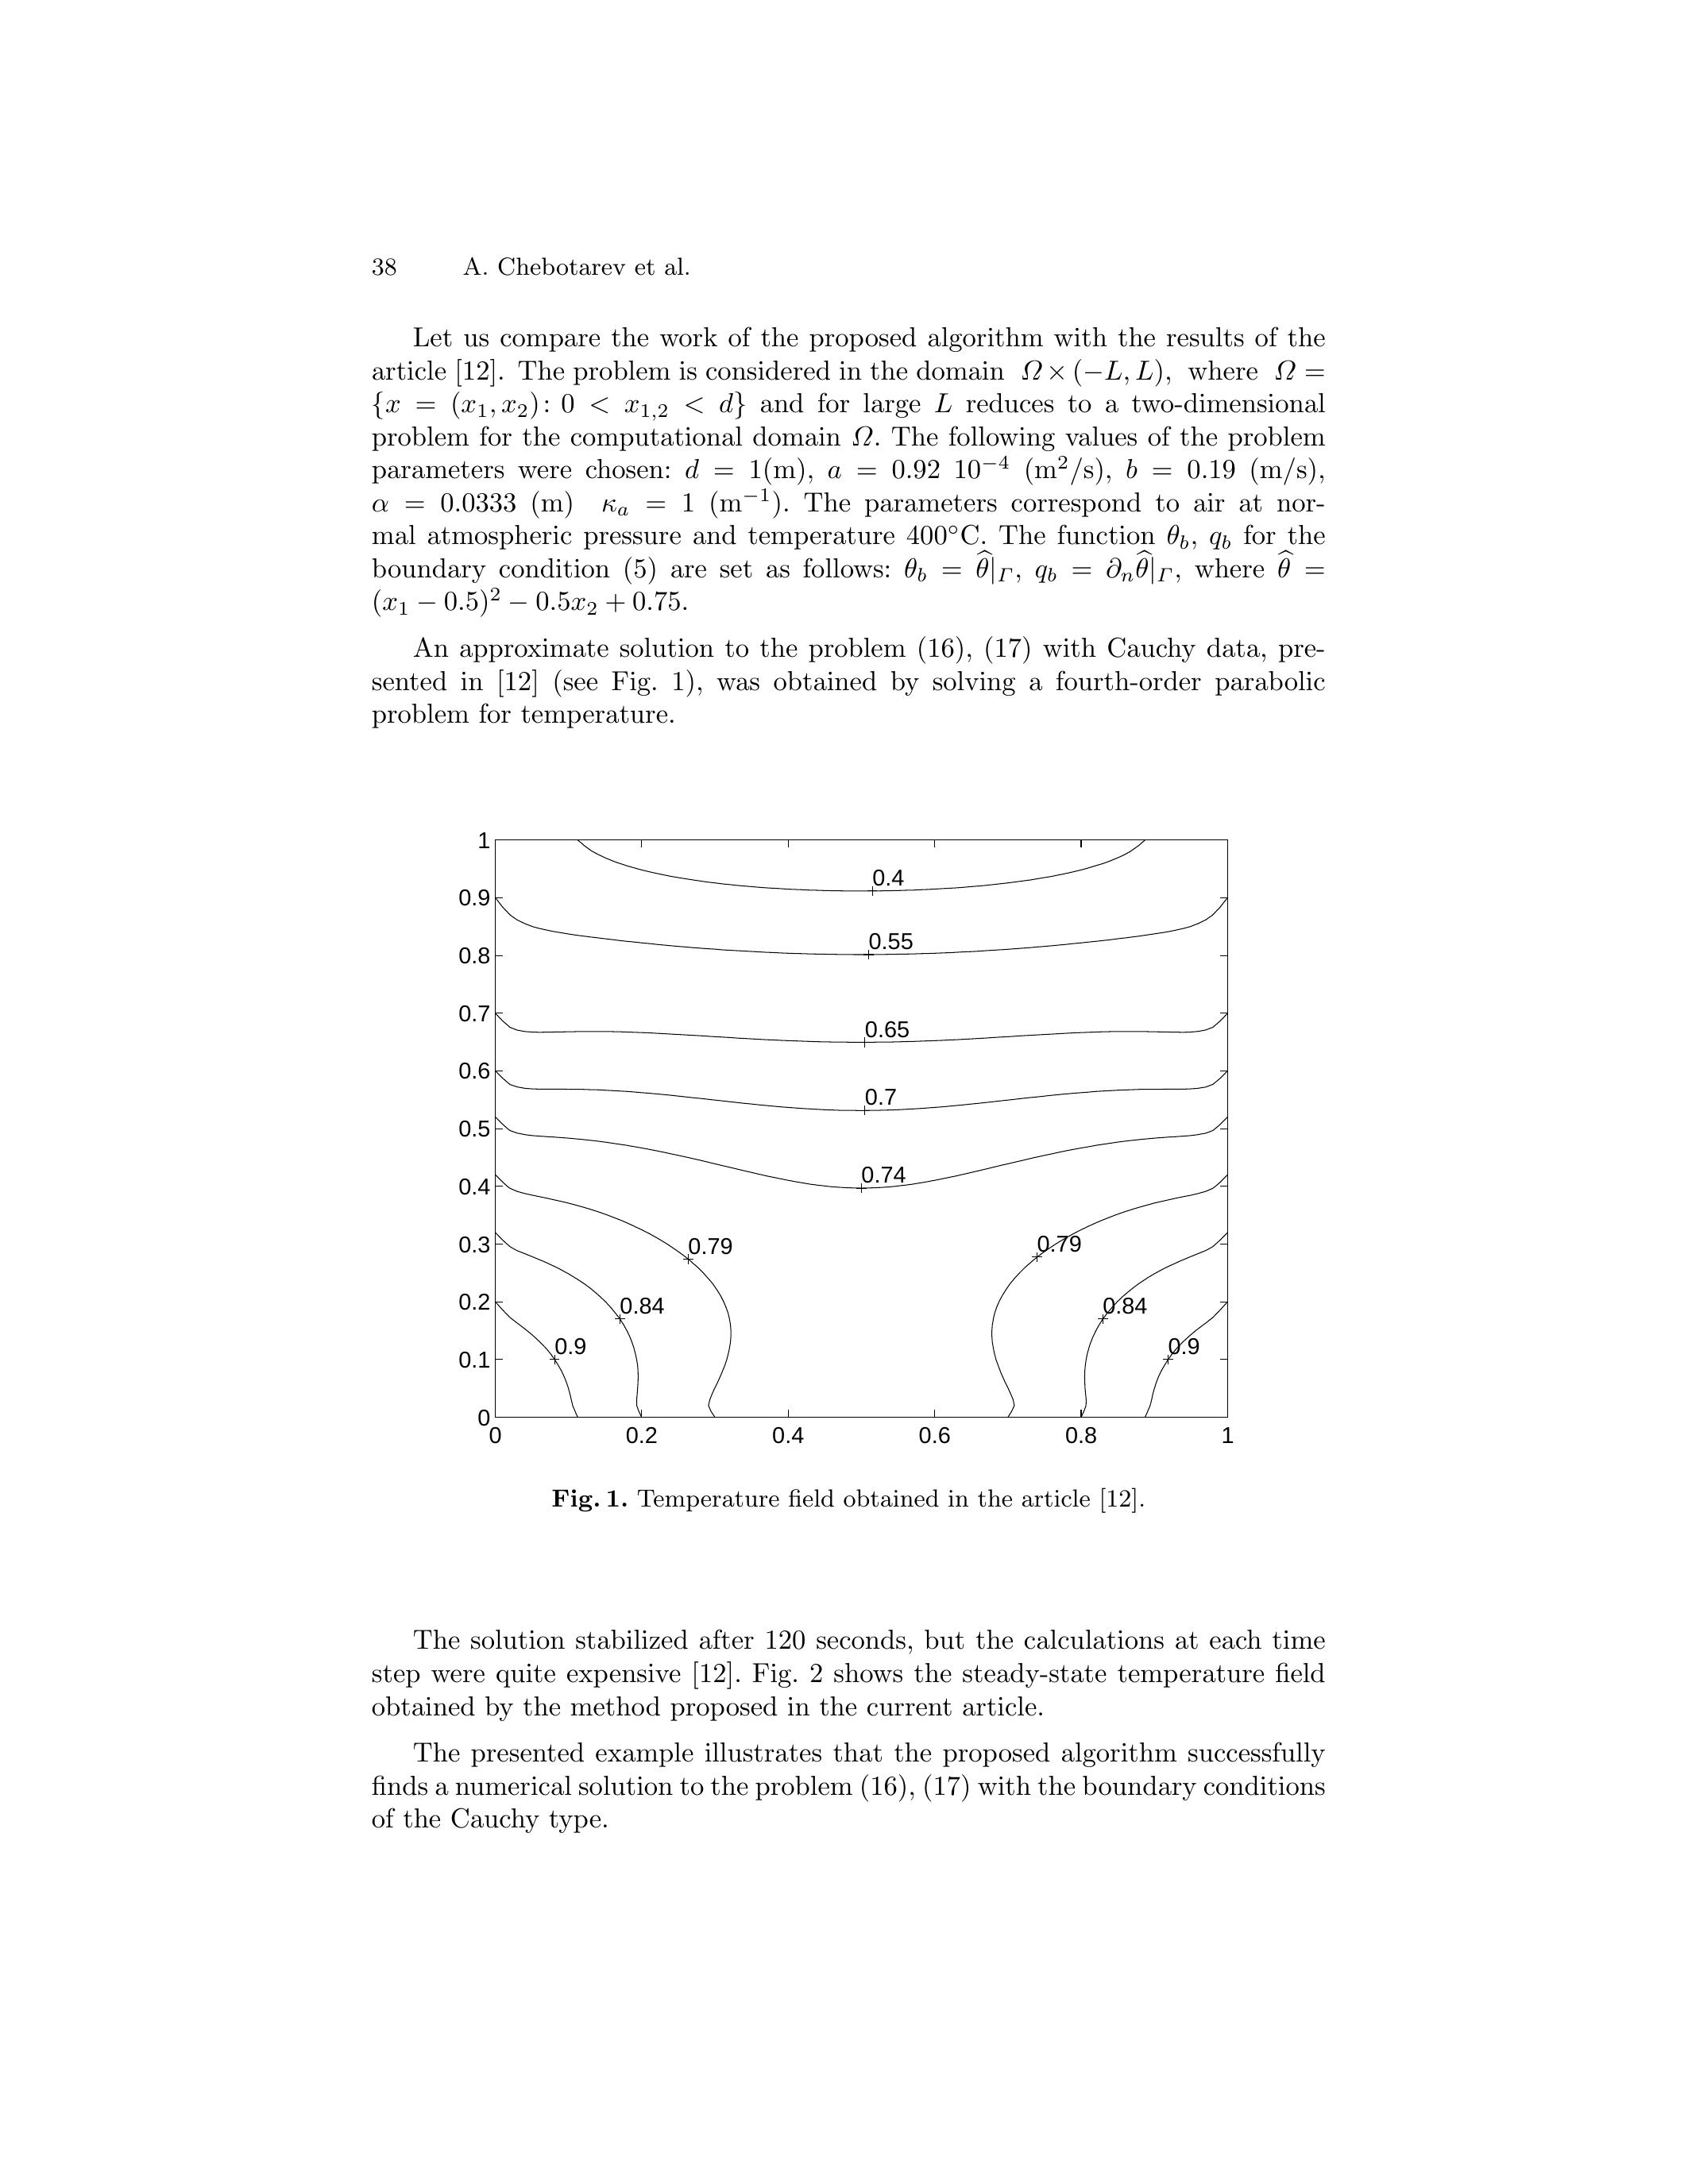
\includegraphics[width=\textwidth]{paper03.png}
\end{center}

Fig. 1. Temperature field obtained in the article [12].

The solution stabilized after 120 seconds, but the calculations at each time step were quite expensive [12]. Fig. 2 shows the steady-state temperature field obtained by the method proposed in the current article.

The presented example illustrates that the proposed algorithm successfully finds a numerical solution to the problem (16), (17) with the boundary conditions of the Cauchy type.
